
% W tym rozdziale opisane będą aspekty języków, przedstawiono informacje o wykorzystanych

% bibliotekach, pokazano fragmenty kodu.


\section{ Aspekty języków }

\subsection{ Popularność języka }
Duża popularność języka zapewnia łatwy dostęp do dużej społeczności osób pracujących nad jego rozwojem. Dla dynamicznie rozwijających się języków powstaje wiele bibliotek, środowisk IDE, narzędzi, a także literatury i przykładów ich zastosowania w rozwiązywaniu konkretnych zadań. Do zastosowania w projektowanych rozwiązaniach warto wybierać języki popularne i nowoczesne, aby uniknąć trudności ze znalezieniem specjalistów do pracy nad projektem. 

\subsection{ Dostępność bibliotek }
Dla otwartych języków programowania powstaje wiele narzędzi i bibliotek, z których duża część jest udostępniana społeczności na różne sposoby. Dla rozwiązań komercyjnych bibliotek jest mniej, natomiast ich jakość najczęściej jest bardzo wysoka, dokumentacja dopracowana a pomoc techniczna łatwo dostępna. 

\subsection{ Wygoda instalacji }
Instalacja języka wraz ze środowiskiem może różnić się znacznie w zależności od systemu operacyjnego. Języki niższych poziomów integrujące się bardziej z systemem operacyjnym mogą być trudniejsze w instalacji i konfiguracji do pracy z np. kartami graficznymi. 

\subsection{ Stopień wykorzystania GPU }
W modelowaniu sieci głębokich wykorzystanie potencjału kart graficznych ma znaczenie kluczowe dla realizacji wydajnych modeli. 

\subsection{ Koszt licencji }
Większość języków i środowisk jest dostępna na licencji otwartej. Wykorzystanie niektórych języków, bibliotek czy środowisk IDE wiąże się z koniecznością zakupu licencji. Wykorzystanie w celach komercyjnych może wymagać zakupu innej, droższej licencji niż wykorzystanie w celach naukowych. 

\subsection{ Wygoda użytkowania }
W większości języków programowania ogólnego przeznaczenia stosuje się bardzo podobne konstrukcje i pracuje się na podobnych rodzajach danych. Języki programowania wysokiego poziomu bazują na bytach abstrakcyjnych, tworzenie kodu jest łatwe i nie wymaga od programisty znajomości dokładnej budowy komputera, znajomości sposobu działania pamięci czy rodzaju procesora na którym będzie uruchamiany program. Nauka programowania w językach wysokiego poziomu jest dużo szybsza niż w językach niższego poziomu jak np. C++, w którym mamy do czynienia ze ścisłą kontrolą typów przy jednoczesnym występowaniu wskaźników, referencji i ramek stosu, czy też w Asemblerze, do programowania w którym niezbędna jest wiedza nie tylko z zakresu np. sposobów reprezentacji liczb w pamięci, przeliczaniu z systemów szesnastkowych na dziesiętne, ale także z zakresu pracy na rejestrach, stosie, wywołaniach przerwań systemowych czy odwołań do funkcji systemu operacyjnego.  \newpage

\section{Python}

\begin{figure}[h]
    	\centering 
            \includegraphics[width=0.9\linewidth]{rysunki/LANG_python.jpg} 
            \caption{Zestawienie aspektów języków }
\end{figure} 
Według bulldogjob.pl najpopularniejszym językiem programowania jest Python \cite{popularnoscJezykow}. Jest to język młody, jednak prężnie rozwijany i bardzo modny. Składa się na to kilka przyczyn. Po pierwsze - jest to język darmowy  (z wyjątkiem specjalistycznych bibliotek). Po drugie - ma bardzo niski próg wejścia. Aby pisać kod w Pythonie, nie trzeba posiadać specjalistycznej wiedzy technicznej ani szczegółowo znać budowy komputera. Naukę programowania w tym języku rozpoczynają już dzieci w wieku szkolnym. Pisanie kodu jest bardzo przyjemne, w kontrolowaniu typów zmiennych pomagają biblioteki narzędziowe. Społeczność użytkowników jest bardzo pomocna, a w sieci znajdziemy dużo przykładów, samouczków i dokumentacji. Istnieje dużo bibliotek, także bibliotek do tworzenia modeli sieci neuronowych. 
Dla poznawania, trenowania modeli AI nadaje się idealnie.
Niestety instalacja systemu z obsługą najnowocześniejszych kart graficznych może być kłopotliwa.


\subsection{Conda, Anaconda, wirtualne środowiska}
Istnieje wiele rozwiązań pomagających zainstalować środowisko, a także budować wiele wirtualnych środowisk na jednej maszynie.

\subsection{Tensorflow}
Biblioteka Tensorflow wymaga rekompilacji do współpracy z GPU. Wersja instalowana z pakietów współpracuje z CPU i wykorzystuje rozkazy procesora AVX. Sprawia trudności przy instalacji, 

\subsection{Scikit-learn}

\subsection{PyTorch}
Wygodna do zainstalowania, bardzo współpracuje bardzo dobrze z procesorami graficznymi zarówno od NVidia, ale także może wykorzystać karty AMD. 







\section{Matlab}
Środowisko Matlab nie jest ujęte w zestawieniu bulldogjob.pl \cite{popularnoscJezykow}. Jest to środowisko płatne, tworzone i wykorzystywane przez środowiska akademickie. Jest przykładem wzorowej obsługi procesu instalacji oprogramowania i wsparcia obsługi kart graficznych. Pisanie kodu jest wygodne, a dostarczona dokumentacja i przykłady są obszerne i wygodne w użyciu. Jedynym, co może być mylące jest rozpoczynanie indeksów od 1. \newline
Dodatek Parallel computing w Matlab umożliwia wykonywanie obliczeń równolegle, w osobnych wątkach, procesach, a także z wykorzystaniem kart graficznych (obecnie tylko NVidia). Dodatki Optimalization Toolbox i Optimalization Computing Toolbox optymalizują tworzony kod, dzięki czemu zwiększają jego wydajność. Dodatek Deep Learning Toolbox dostarcza gotowych metod do obliczeń sieci neuronowych.

\section{C++}
Język C/C++ wg. bulldogjob.pl osiąga popularność na poziomie 6.6\% \cite{popularnoscJezykow}. C++ jest językiem, który nieco traci popularność na korzyść np. Pythona czy Rust. Jest to język darmowy, a integracja ze sterownikami i bibliotekami kart graficznych jest natywna. Idealnie pracuje w systemach Linux, ale dobrze działa także w Windows z Microsoft Visual Studio.
Jest to język kompilowany, w którym budowanie programu trwa dłużej niż w Pythonie czy Matlabie, jednak skompilowana aplikacja działa bardzo szybko. Język ten dobrze obsługuje karty graficzne. Jednak stawia duże wymagania użytkownikowi piszącemu kod. Do dobrego wykorzystania potencjału wymaga rozumienia procesów zachodzących w sprzęcie, znajomości wielu pojęć języka oraz dobrego poruszania się w typach danych. 

\section{Java}
Według bulldogjob.pl wskaźnik popularności dla języka Java wynosi 26.2\% \cite{popularnoscJezykow}. Java jest językiem podobnym do C++, jest to język kompilowany do kodu bajtowego uruchamianego w maszynie wirtualnej. Ma ścisłą kontrolę typów. Niektóre wersje wymagają opłacenia licencji, większość jednak jest darmowa. Wykonywalny kod działa dość szybko, nieco wolniej niż C++. Instalacja wymaga nieco uwagi. Istnieją biblioteki umożliwiające wsparcie obliczeń na kartach graficznych, jednak w tej pracy nie wykorzystywano tych bibliotek. Jest rzadko wykorzystywany do modelowania sieci neuronowych. 
~ \newpage


\section {Podsumowanie i wnioski}
\begin{figure}[h]
    	\centering 
            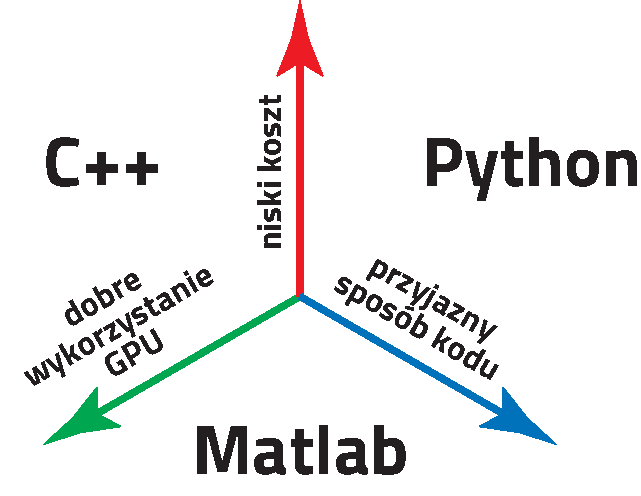
\includegraphics[width=0.5\linewidth]{rysunki/lang.jpg} 
            \caption{ Priorytety przy wyborze języka }
\end{figure} 
Przy wyborze języka trzeba zdecydować się na dwa z trzech priorytetów, jeden niestety trzeba odrzucić. Najwydajniejsze języki to C++ i Matlab. Najwygodniej pracuje się w Pythonie więc jest najczęściej wybierany do tworzenia modeli w celach  badawczych. Duże produkcyjne modele powstają zwykle w języku C/C++ i są uruchamiane w środowiskach serwerowych. 

\section{Dodatkowe wnioski}

\subsection{Zadanie 3}
Zbliżone czasy wykonania zadania 3 dla PyTorch z użyciem GPU i bez - sugerują, że możliwości GPU nie zostały użyte prawidłowo.

Poprawa kodu powoduje zdecydowane skrócenie czasu wykonania, jednocześnie zmienia wnioski wynikające z zestawienia: 

\begin{lstlisting}
-------------
CUDA available. Using GPU acceleration.
cuda
(59400, 1, 28, 28)
tensor([13.2702, -8.9589,  2.4638,  0.5280, -4.6336,  
  2.0661,  0.6992,  0.2631, 0.6639,  0.2546], 
  device='cuda:0', grad_fn=<SelectBackward0>)
  
# Python PyTorch 2.0 60000 Images, 100 Epoch 
  Time:  29.587559938430786
  Test accuracy: 0.6212121248245239
------------------
\end{lstlisting}